\documentclass[onecolumn,10pt]{jhwhw}

\usepackage{epsfig} %% for loading postscript figures
\usepackage{amsmath}
\usepackage{graphicx}
\usepackage{grffile}
\usepackage{pdfpages}
\usepackage{algpseudocode}
\usepackage{wrapfig}
\usepackage{pgfplots}
\usepackage{amsfonts}
\usepackage{booktabs}
\usepackage{siunitx}
\usepackage{commath}
\usepackage{rotating}

% Default fixed font does not support bold face
\DeclareFixedFont{\ttb}{T1}{txtt}{bx}{n}{12} % for bold
\DeclareFixedFont{\ttm}{T1}{txtt}{m}{n}{12}  % for normal

% Custom colors
\usepackage{color}
\usepackage{listings}
\usepackage{framed}
\usepackage{caption}
\usepackage{bm}
\captionsetup[lstlisting]{font={small,tt}}

\definecolor{mygreen}{rgb}{0,0.6,0}
\definecolor{mygray}{rgb}{0.5,0.5,0.5}
\definecolor{mymauve}{rgb}{0.58,0,0.82}

\lstset{ %
  backgroundcolor=\color{white},   % choose the background color; you must add \usepackage{color} or \usepackage{xcolor}
  basicstyle=\ttfamily\footnotesize, % the size of the fonts that are used for the code
  breakatwhitespace=false,         % sets if automatic breaks should only happen at whitespace
  breaklines=true,                 % sets automatic line breaking
  captionpos=b,                    % sets the caption-position to bottom
  commentstyle=\color{mygreen},    % comment style
  deletekeywords={...},            % if you want to delete keywords from the given language
  escapeinside={\%*}{*)},          % if you want to add LaTeX within your code
  extendedchars=true,              % lets you use non-ASCII characters; for 8-bits encodings only, does not work with UTF-8
  frame=single,                    % adds a frame around the code
  keepspaces=true,                 % keeps spaces in text, useful for keeping indentation of code (possibly needs columns=flexible)
  columns=flexible,
  keywordstyle=\color{blue},       % keyword style
  language=Python,                 % the language of the code
  morekeywords={*,...},            % if you want to add more keywords to the set
  numbers=left,                    % where to put the line-numbers; possible values are (none, left, right)
  numbersep=5pt,                   % how far the line-numbers are from the code
  numberstyle=\tiny\color{mygray}, % the style that is used for the line-numbers
  rulecolor=\color{black},         % if not set, the frame-color may be changed on line-breaks within not-black text (e.g. comments (green here))
  showspaces=false,                % show spaces everywhere adding particular underscores; it overrides 'showstringspaces'
  showstringspaces=false,          % underline spaces within strings only
  showtabs=false,                  % show tabs within strings adding particular underscores
  stepnumber=1,                    % the step between two line-numbers. If it's 1, each line will be numbered
  stringstyle=\color{mymauve},     % string literal style
  tabsize=4,                       % sets default tabsize to 2 spaces
}

\author{John Karasinski}
\title{}

\begin{document}
%\maketitle

\noindent {\large \bfseries Homework v1}
\begin{enumerate}
\item Technical requirements list and flowchart
\item Product breakdown structure for vehicle
\item List of required analyses \\
\end{enumerate}

\noindent We can directly convert the first draft of the Customer Expectations into technical requirements. The Customer Expectations/Mission Requirements v1 state that the reboost vehicle must:\\

\begin{enumerate}
\item Launch on an existing US launcher from Cape Canaveral into the HST orbit
\begin{description}
  \item[Requirement 1] \hfill \\
  Reboost vehicle must be launched on existing US launcher from Cape Canaveral into the HST orbit.

  \item[Requirement 2] \hfill \\
  Reboost vehicle must be able to withstand temperature conditions of launch and orbit.
  \item[Requirement 3] \hfill \\
  Reboost vehicle must be able to withstand vibration conditions and g-loading of launch.

\end{description}
\item Rendevous and dock with HST using robotic-arm grapple fixture
\begin{itemize}
\item Use HST or rebooster ADCS to orient combined spacecraft for reboost
\begin{description}
  \item[Requirement 4] \hfill \\
  Reboost vehicle must communicate with HST to orient combined spacecraft.
\end{description}
\item Reboost thrust must result in solar array boom deflection of no more than 50cm
\begin{description}
  \item[Requirement 5] \hfill \\
  Reboost vehicle thrust must not cause a solar array boom deflection of more than 50cm.
\end{description}
\item Undock from HST and destructively de-orbit into atmosphere
\begin{description}
  \item[Requirement 6] \hfill \\
  Reboost vehicle must have sufficient fuel to dock and reboost HST, and de-orbit into atmosphere.
\end{description}
\item Send and receive state-vector, attitude, and system health telemetry to/from HST
\begin{description}
  \item[Requirement 7] \hfill \\
  Reboost vehicle must be able to exchange information with HST.
\end{description}
\item Send and receive state-vector, attitude, and system health telemetry to/from NASA Mission Control Center (MCC), either directly, or indirectly via HST and or TDRS satellites
\begin{description}
  \item[Requirement 8] \hfill \\
  Reboost vehicle should be able communicate with TDRS in case of communication failure with HST.
\end{description}
\item Be able to recover from one Single Event Upset per hour in the onboard Command and Control Computer
\begin{description}
  \item[Requirement 9] \hfill \\
  Reboost vehicle must be able to recover from one Single Event Upset per hour in the onboard Command and Control Computer.
\end{description}
\item No requirement on duration of mission
\item Power and thermal requirements not specified – to be determined by design to meet mission objectives
\begin{description}
  \item[Requirement 10] \hfill \\
  Reboost vehicle must have sufficent power and thermal specifications to meet mission objectives.
\end{description}
\item Main body of spacecraft bus must include MMOD shielding (impact spec TBD)
\begin{description}
  \item[Requirement 11] \hfill \\
  Reboost vehicle must include bus with MMOD shielding (impact spec TBD).
\end{description}
\item ADCS must be able to recover from/override both jet-fail-on, and jet-fail cases during proximity operations without collision of mission failure
\begin{description}
  \item[Requirement 12] \hfill \\
  Reboost vehicle ADCS system must be able to recover from/override both jet-fail-on, and jet-fail cases during proximity operations without collision of mission failure.
\end{description}
\item Loss of communications between rebooster and HST or MCC must not result in collision
\begin{description}
  \item[Requirement 13] \hfill \\
  Reboost vehicle must not collide with HST.
\end{description}
\end{itemize}
\end{enumerate}

\begin{figure}[h!]
\begin{center}
\rotatebox{90}{
  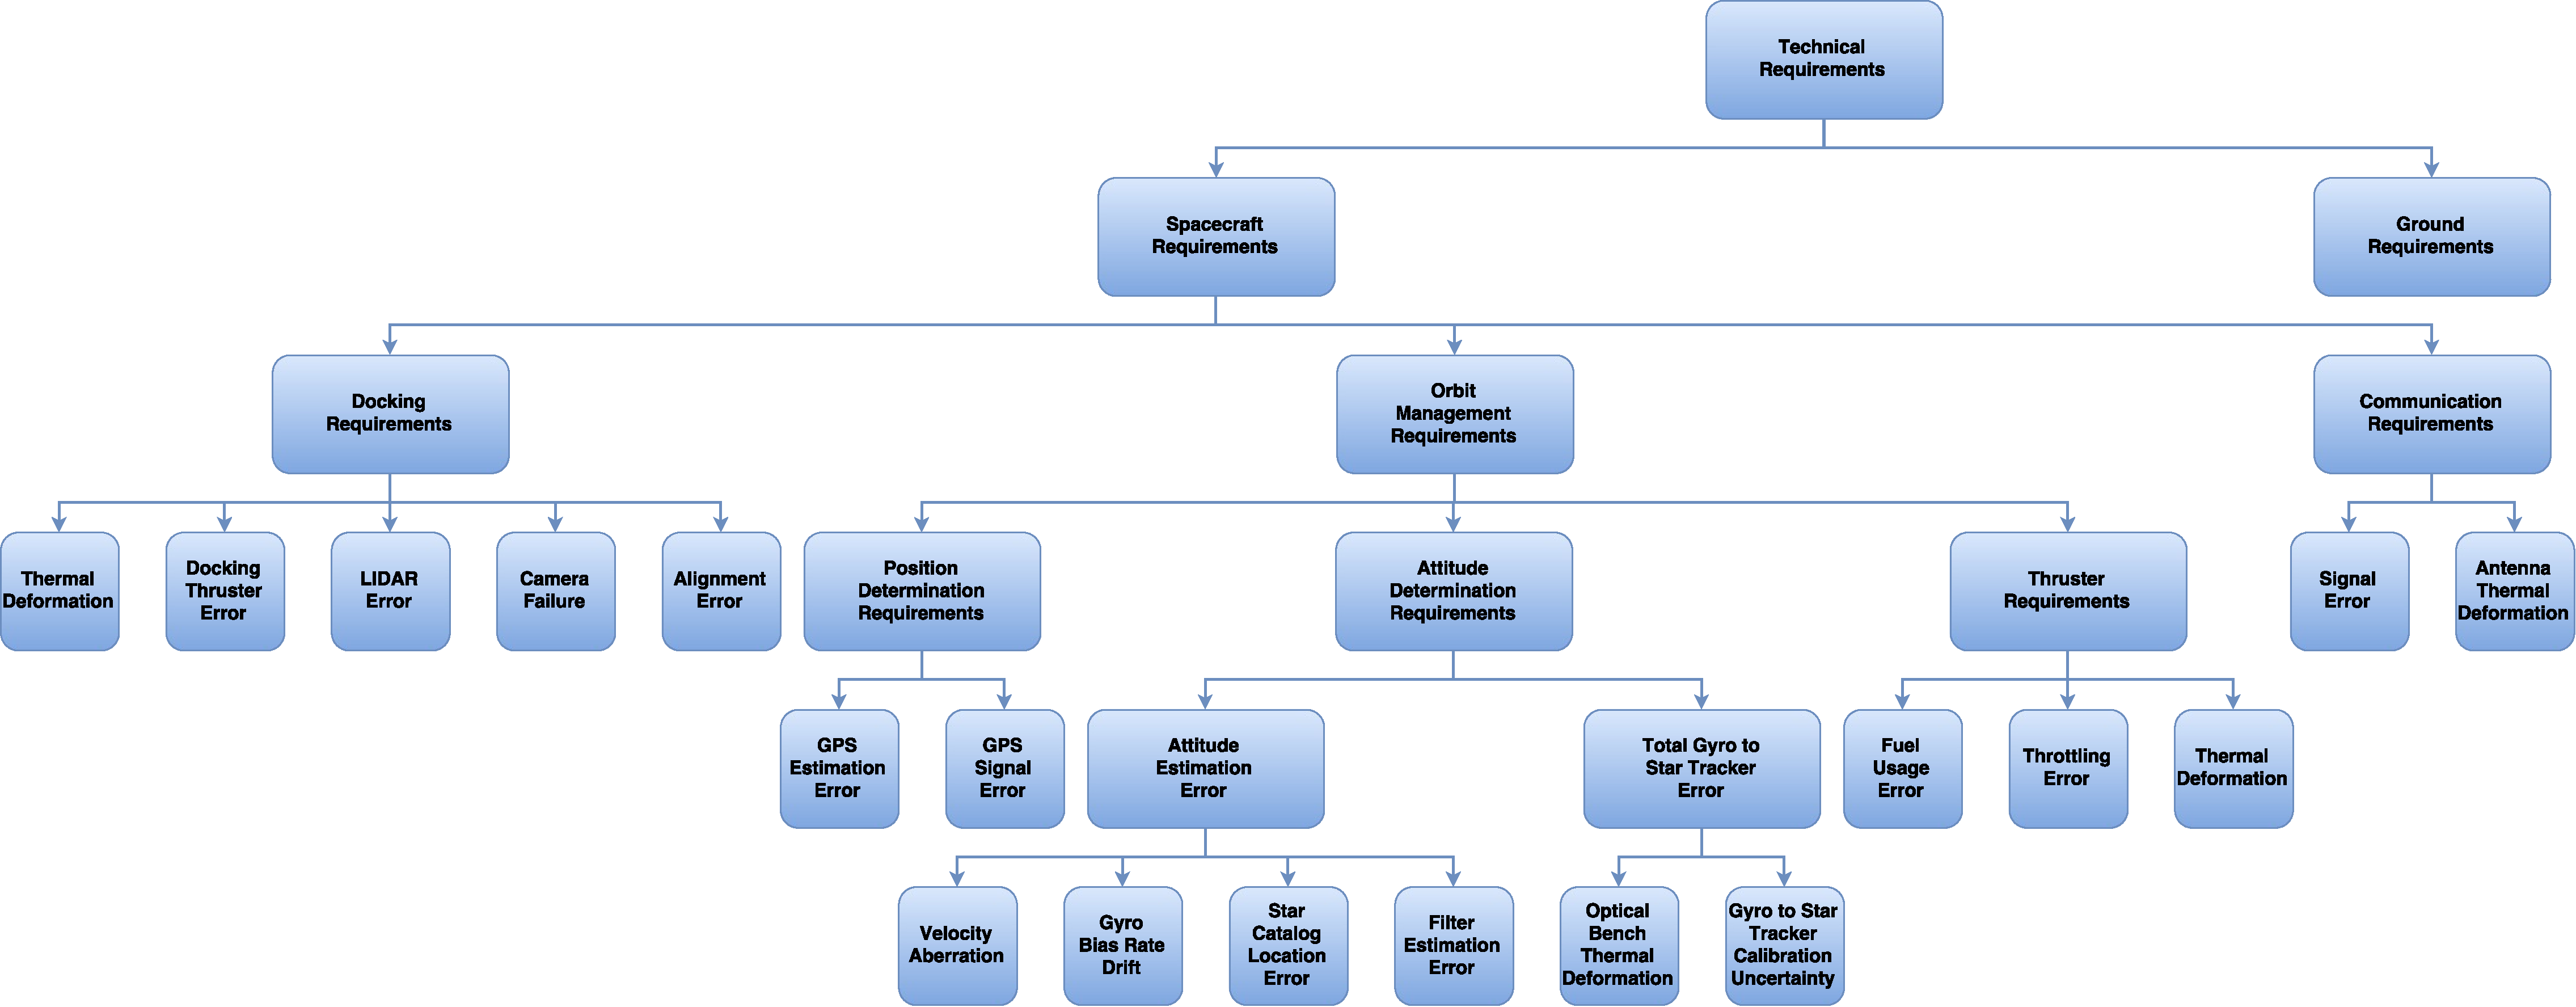
\includegraphics[width=1.3\textwidth]{4.2-4 (Technical Requirements)}
  \label{fig:on}
}
\end{center}
\caption{Technical Requirements}
\end{figure}

\begin{figure}[h!]
\begin{center}
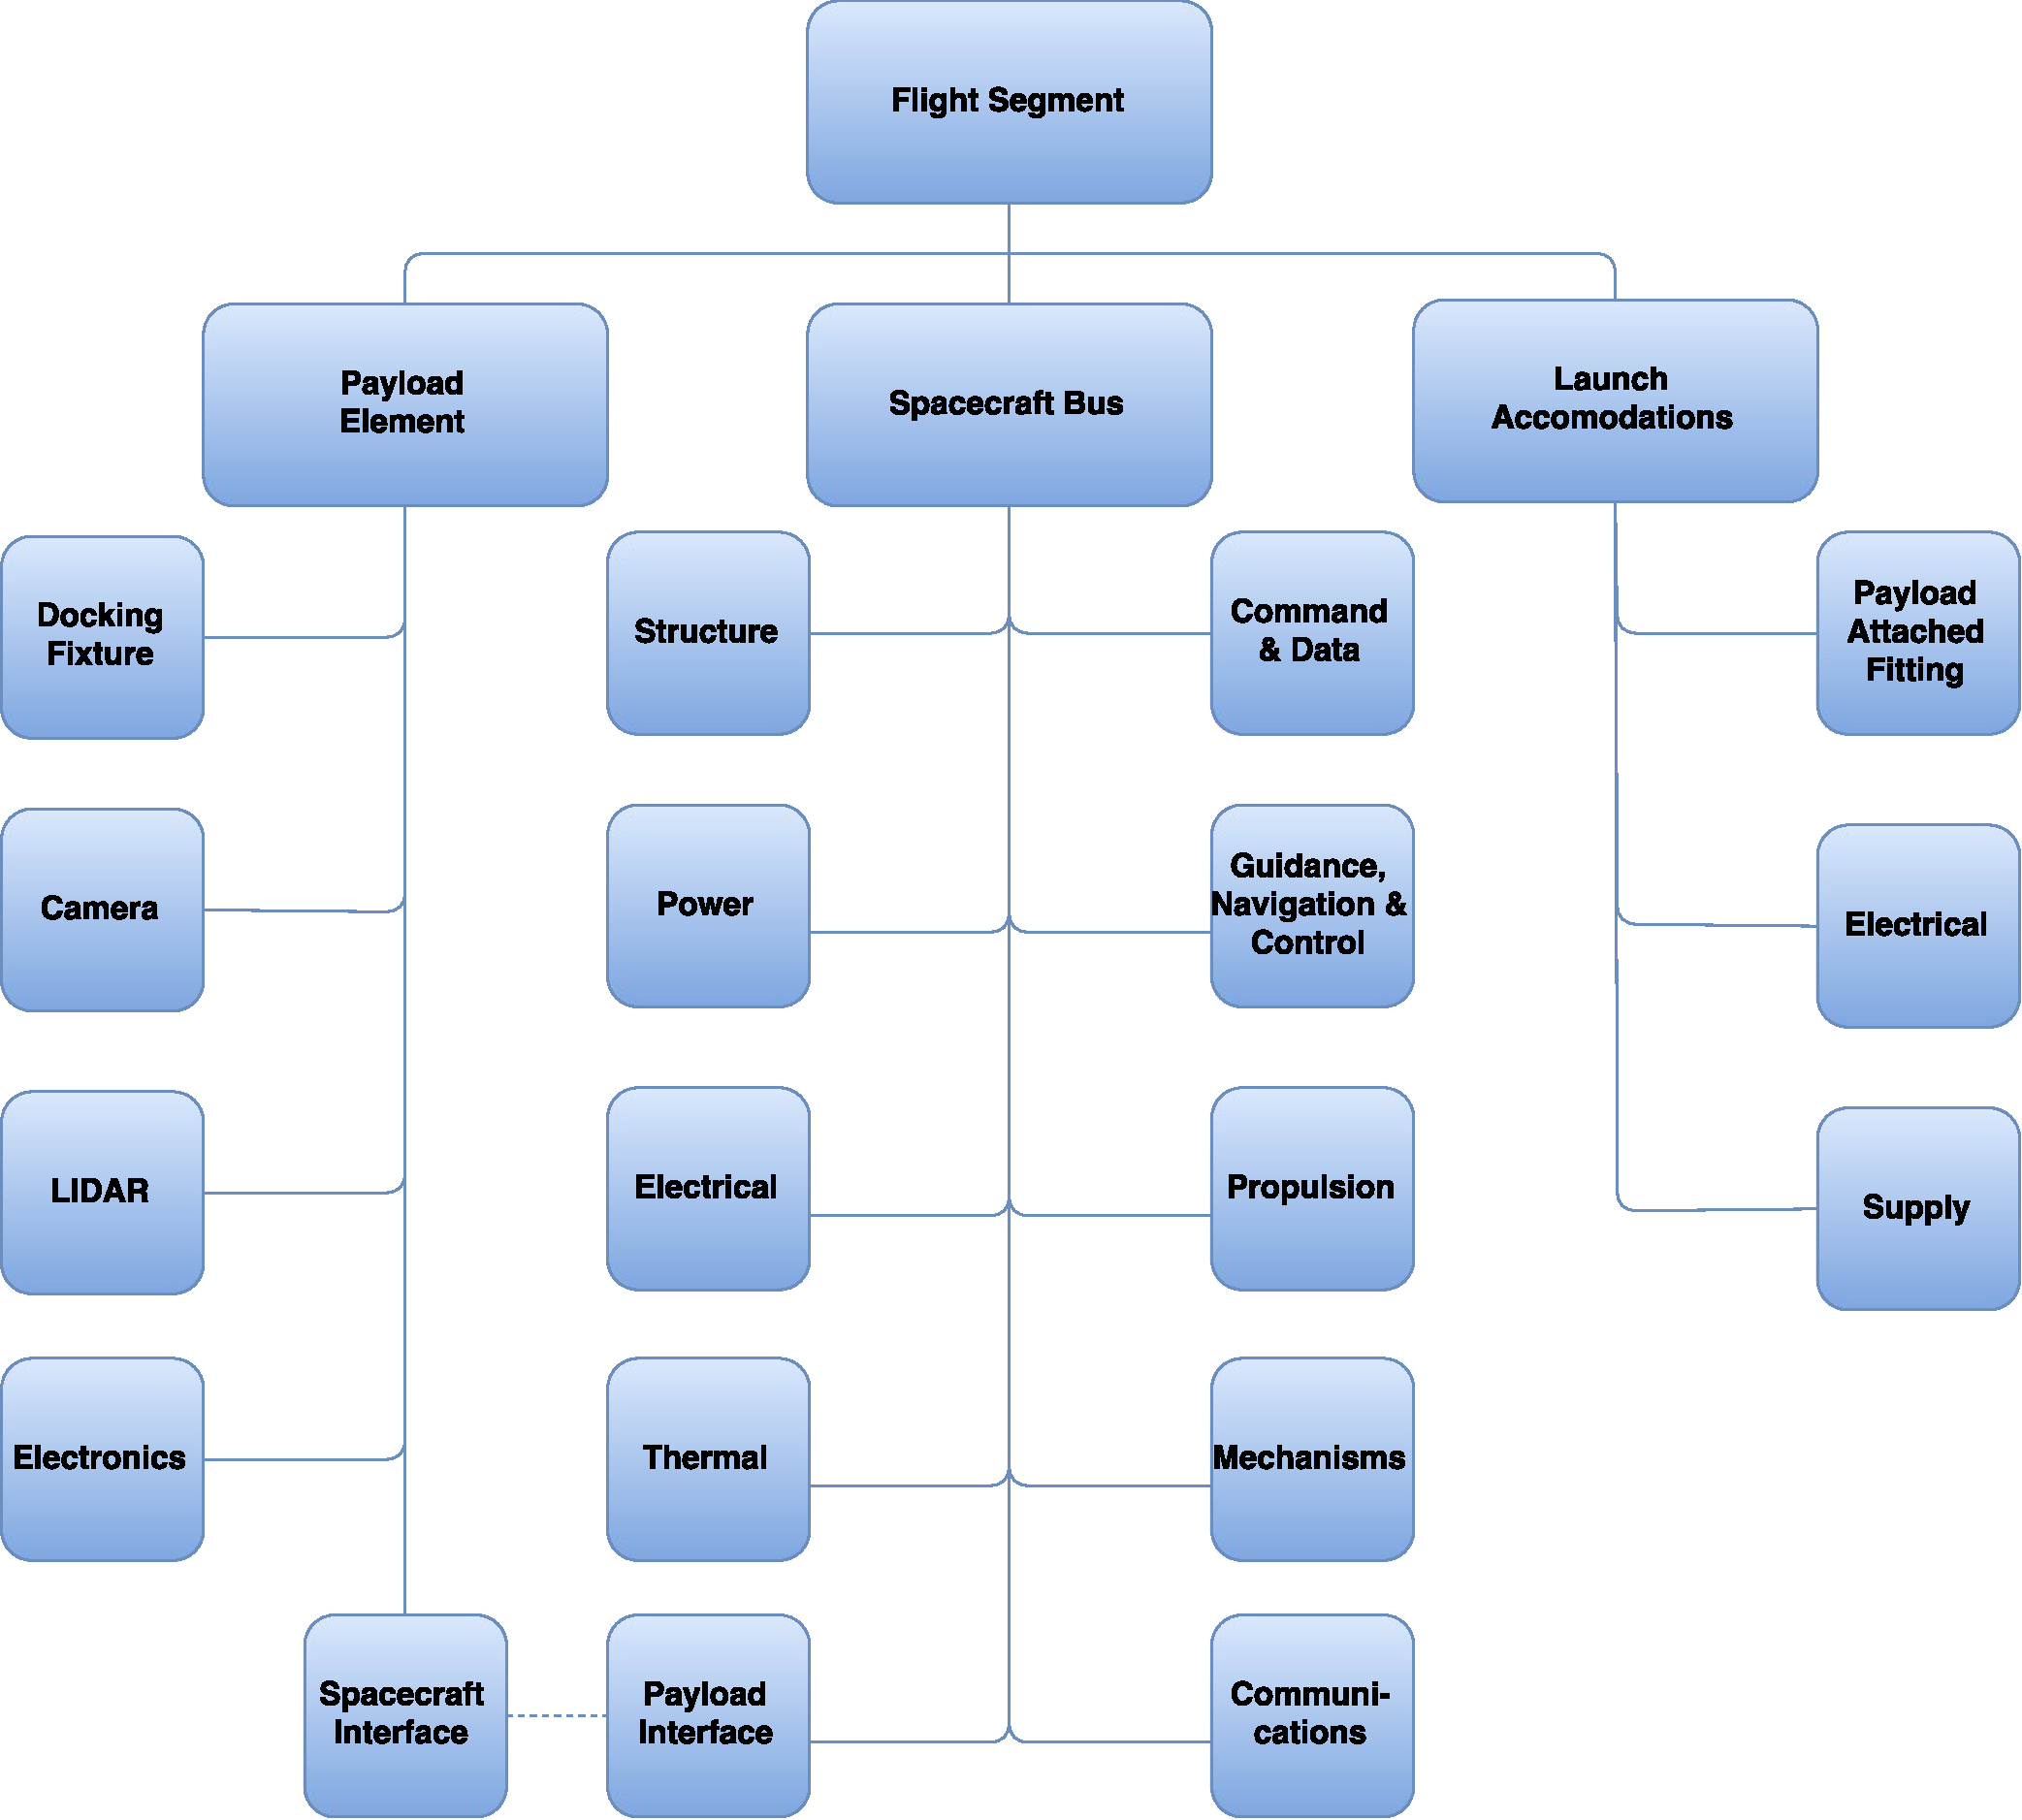
\includegraphics[width=1\textwidth]{4.3-2 (Product Breakdown)}
\label{fig:on}
\end{center}
\caption{Product Breakdown}
\end{figure}

\clearpage
\noindent To complete the mission requirements, analyses must be completed to answer the following questions:
\begin{enumerate}
\item What are the mass requirements for a reboost vehicle to reboost the HST spacecraft to circular orbit so that orbital decay is extended to 5 years beyond the JWST 10/23 launch date, i.e. to 10/28 (currently estimated HST end-of-life is 2020) and then de-orbit in the atmosphere?
\item What existing US launcher can launch an appropriately sized reboost vehicle into the HST orbit?
\item What thermal and vibrational conditions must the spacecraft be able to withstand?
\item How does HST communicate, and how close to HST does the reboost vehicle need to be to communicate with HST?
\item How much force at the robotic-arm grapple fixture point causes a 50cm solar array boom deflection?
\item How do satellites communicate with TDRS, and what kind of power requirements are necessary to do this?
\item What kinds of redundant computer systems are necessary to recover from one Single Event Upset per hour in the onboard Command and Control Computer?
\item How much MMOD shielding is necessary to meet the impact spec?
\item What are the most effective ways to negate jet-fail-on, and jet-fail cases during proximity operations without collision of mission failure?
\end{enumerate}

\end{document}
